\documentclass{beamer}
\usepackage[spanish]{babel}
\usepackage[utf8]{inputenc}
\usepackage{amsmath}
\usepackage{amsthm}
\usepackage{amssymb}
\usefonttheme{serif}
\usepackage{multicol}
\usepackage{graphicx}

\beamertemplatenavigationsymbolsempty

\usepackage[
backend=biber,
style=chem-angew,
sorting=ynt
]{biblatex}
\AtBeginBibliography{\small}

\addbibresource{blb.bib}

\newcommand\blfootnote[1]{%
  \begingroup
  \renewcommand\thefootnote{}\footnote{#1}%
  \addtocounter{footnote}{-1}%
  \endgroup
}

\newcommand{\vol}{\mathrm{vol}}



\title{Desigualdades Discretas del tipo Brunn-Minkowski}
\author{Luis González}
\institute{Instituto de Matemáticas - UNAM}
\titlegraphic{
    
\includegraphics[width=2.5cm]{pics/im.png}
}
%\date{Noviembre 2022}


\AtBeginSection[]
{
  \begin{frame}
    \frametitle{Plan de la plática}
    \tableofcontents[currentsection]
  \end{frame}
}


\begin{document}

\maketitle

%-----------------------
\begin{frame}{Los protagonistas}
    \begin{figure}
\begin{multicols}{2}
    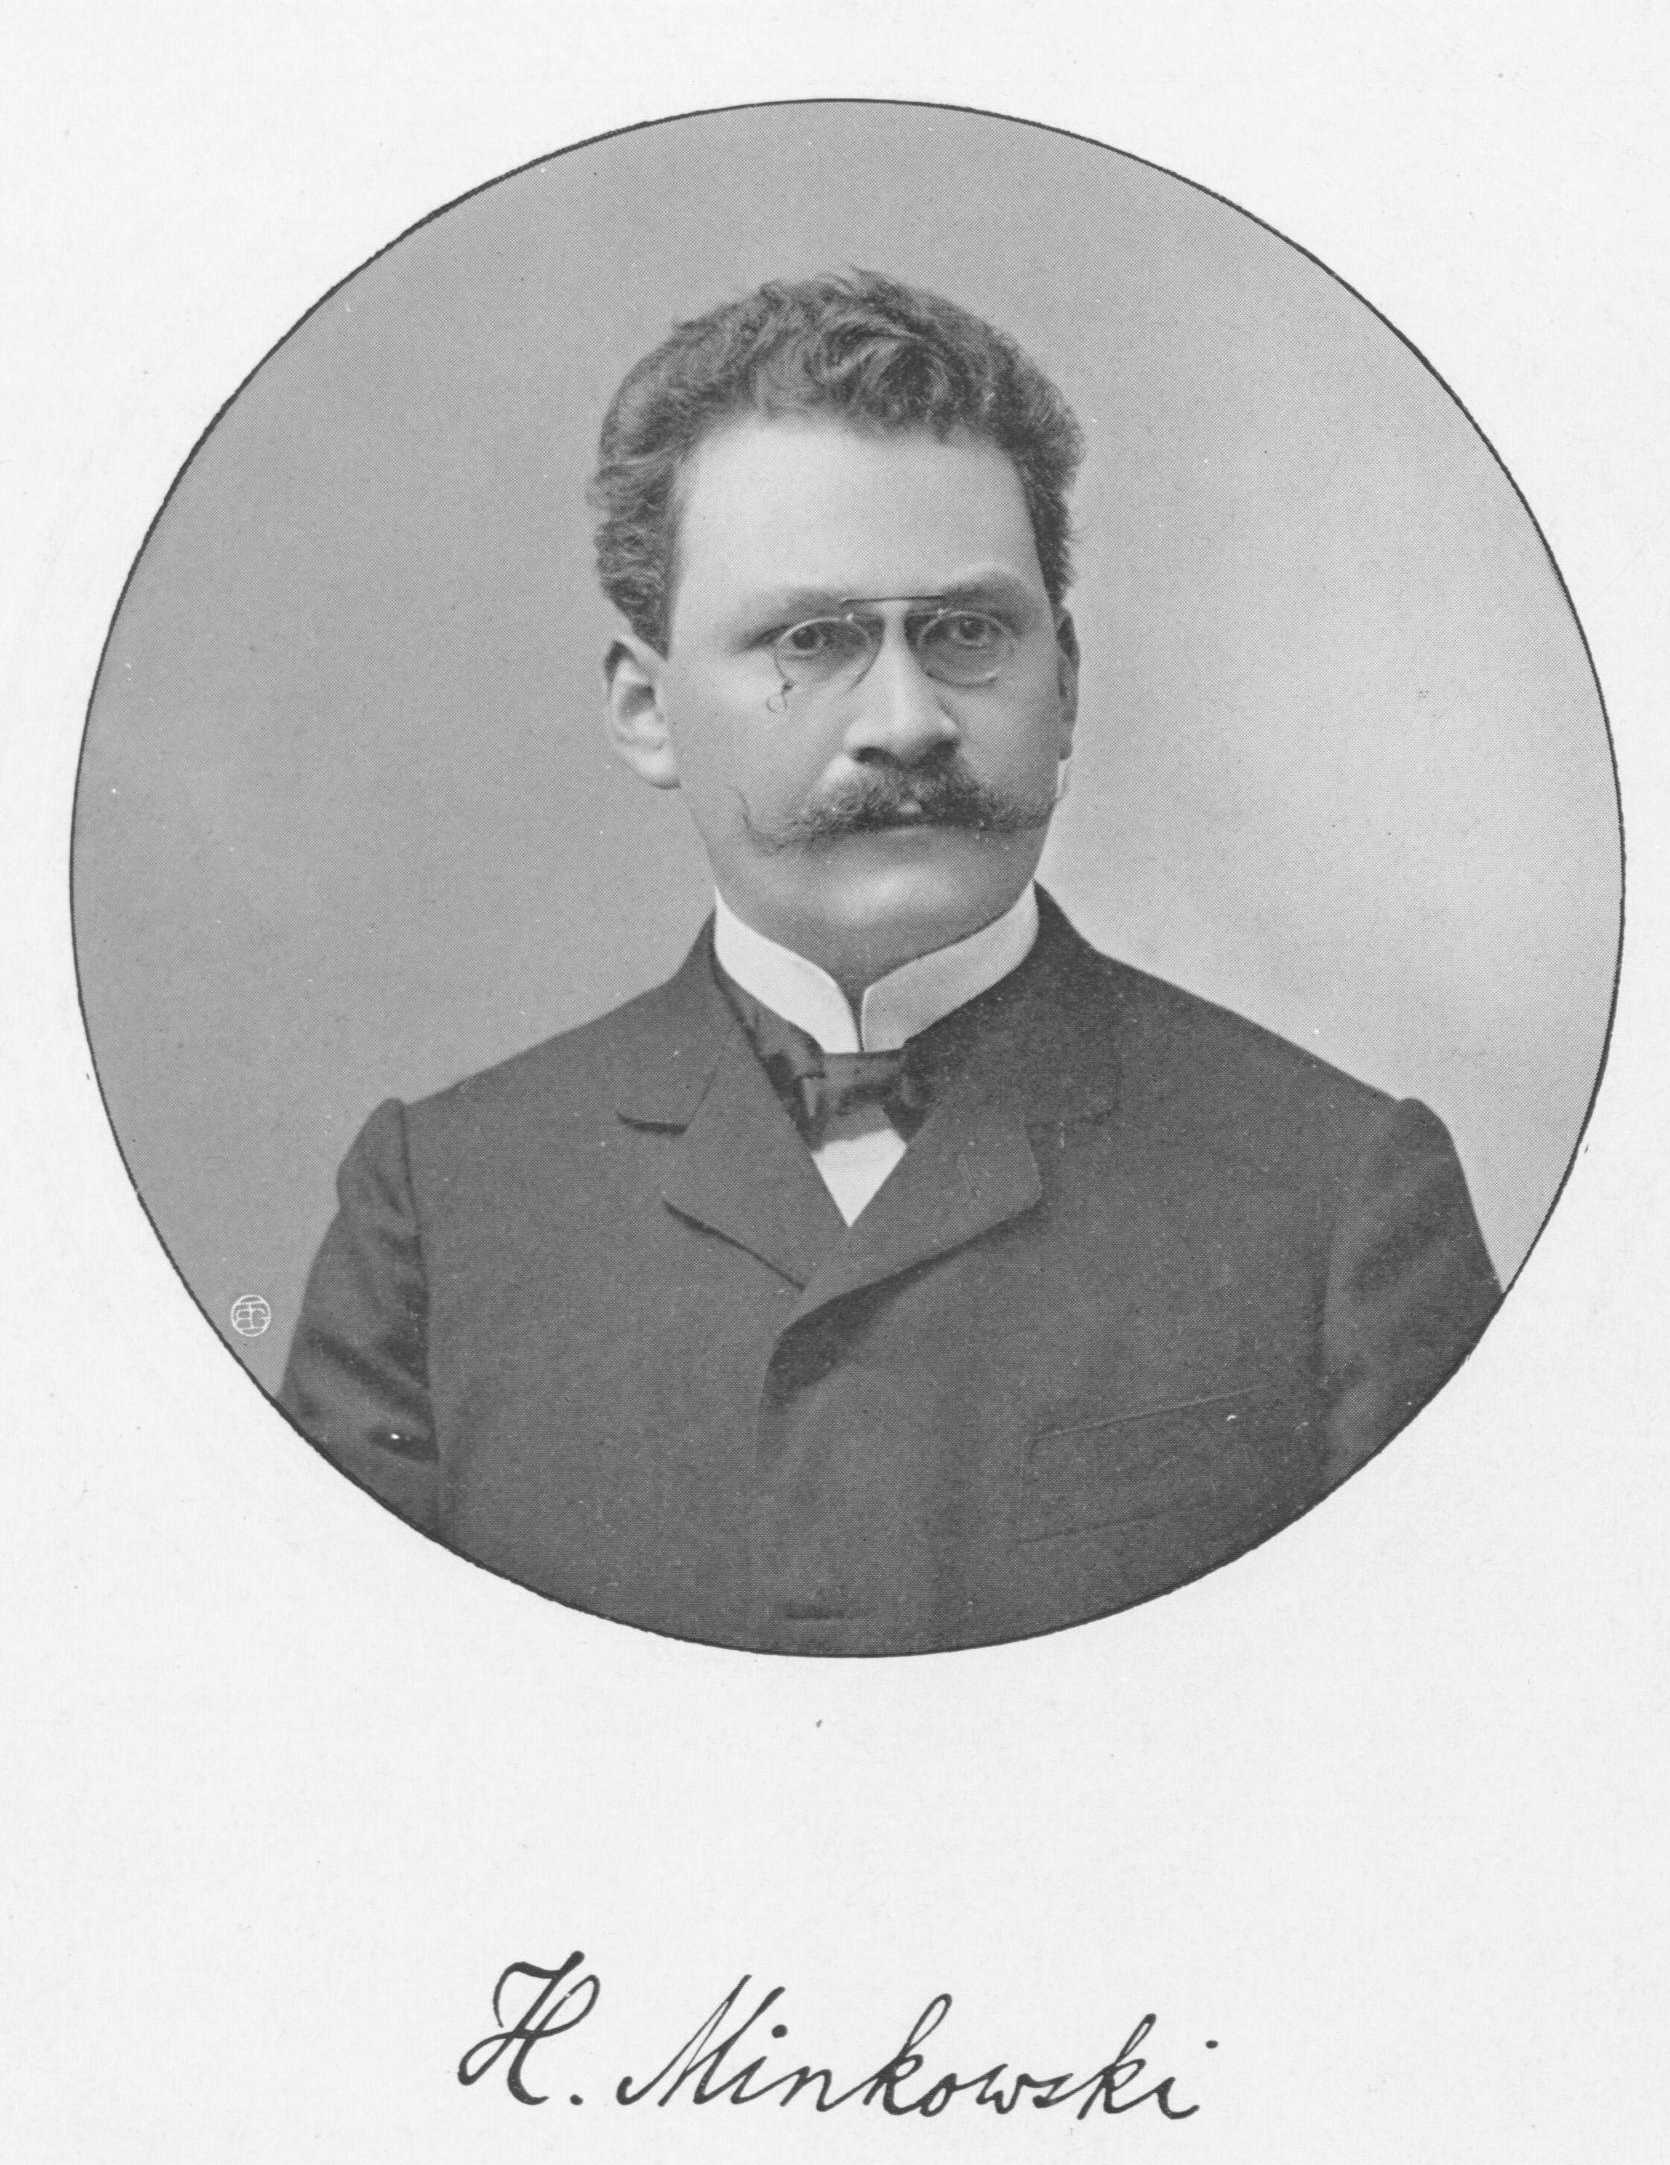
\includegraphics[width=\linewidth]{pics/minkowski.jpg}\par 
    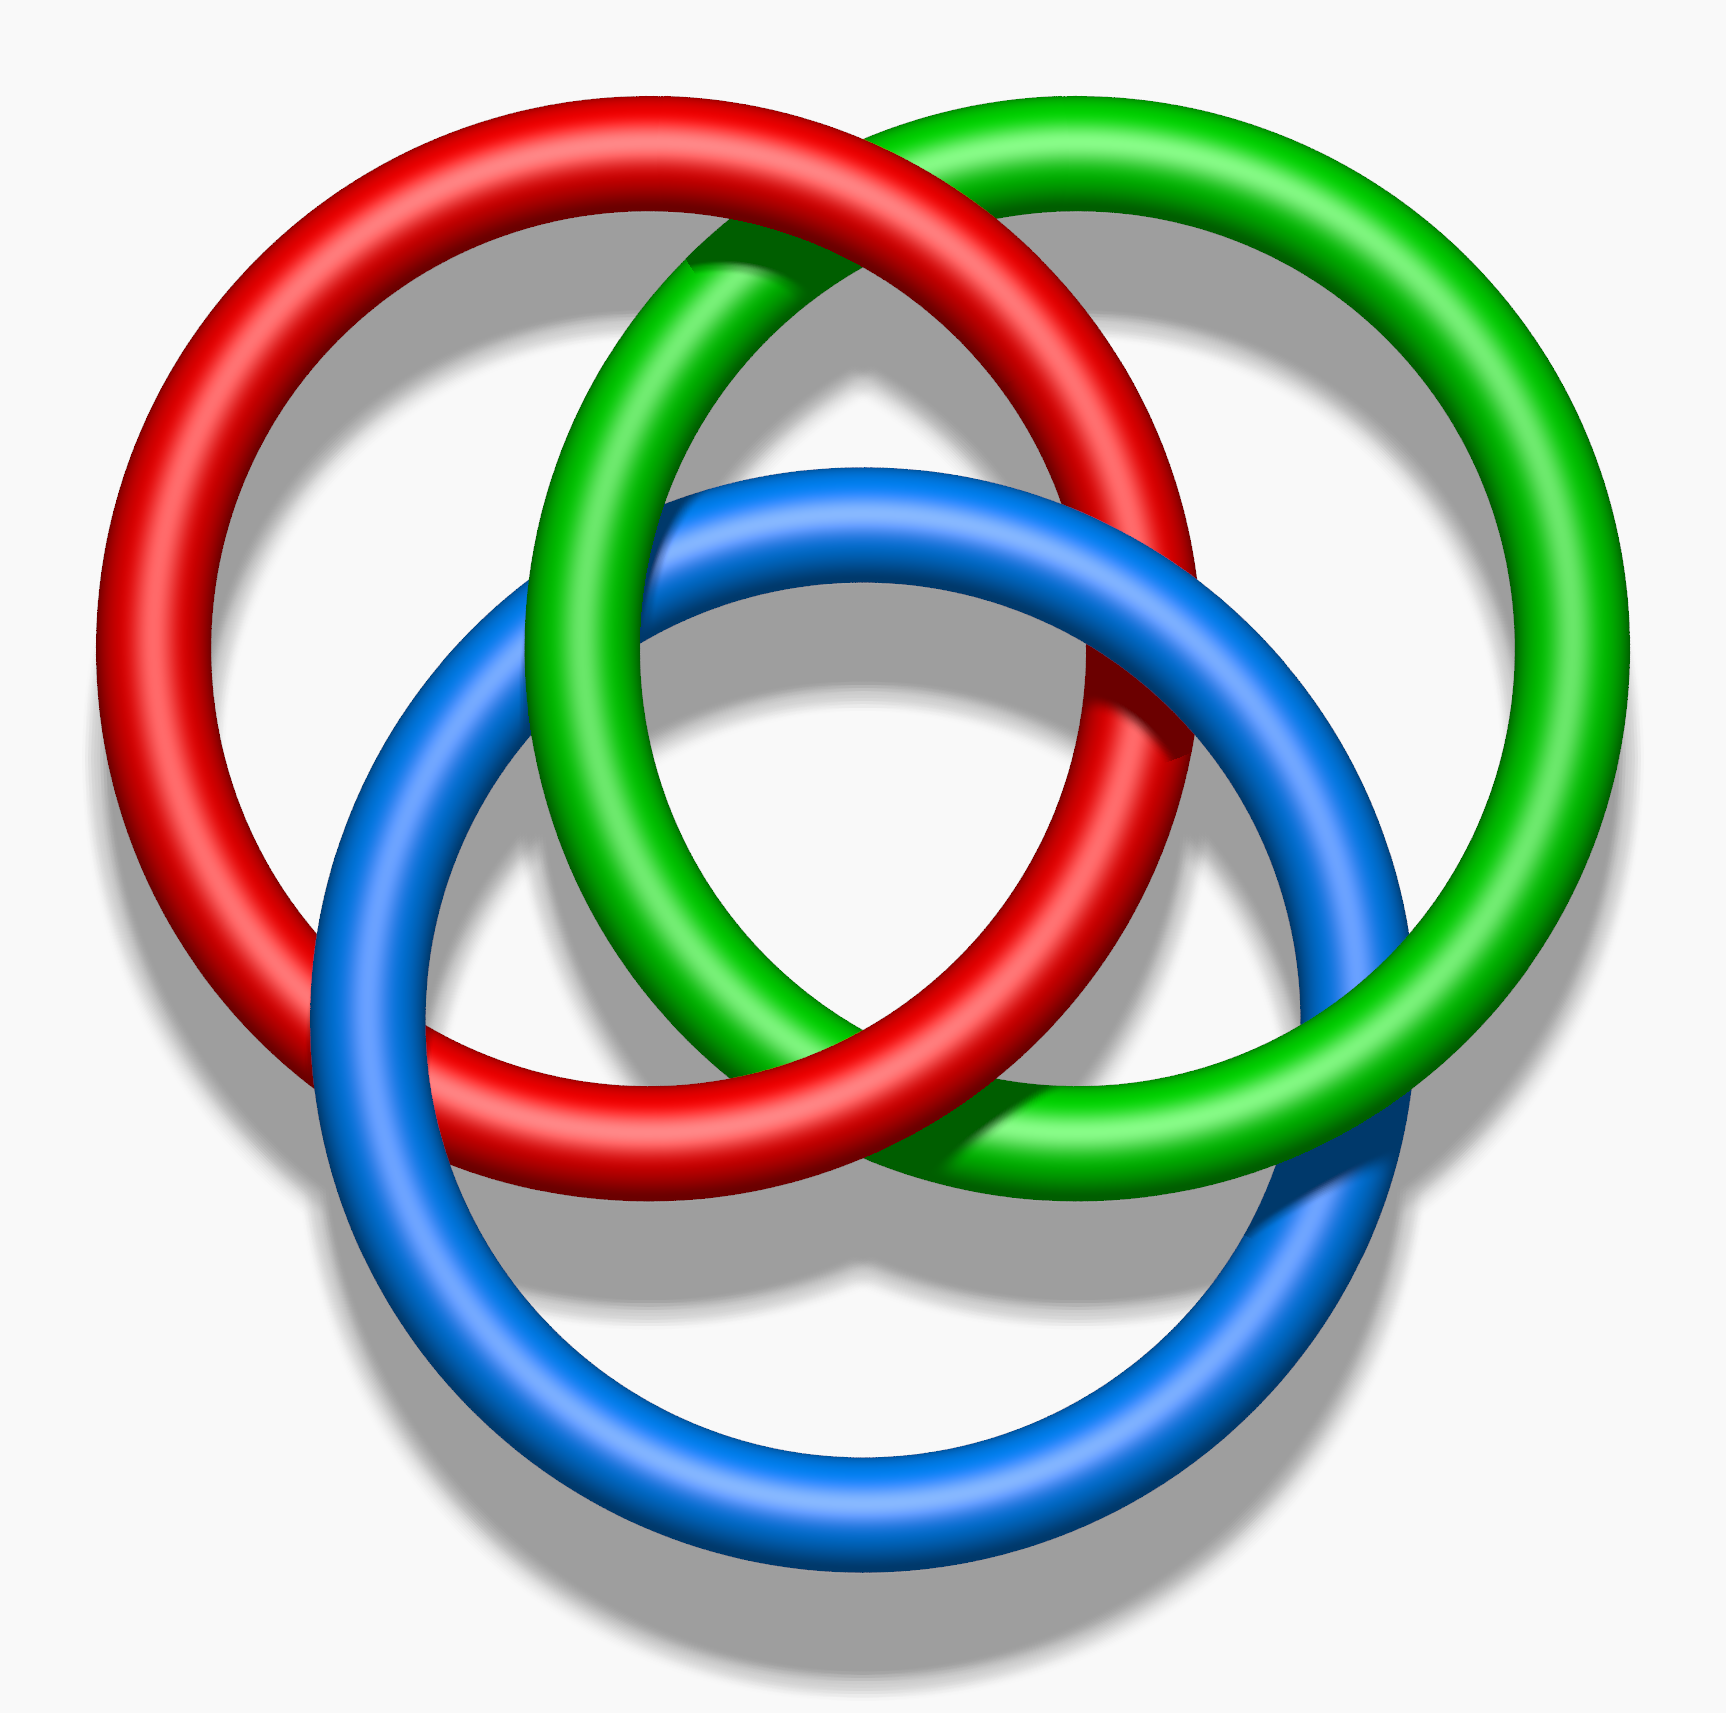
\includegraphics[width=\linewidth]{pics/rings.png}\par 
    \end{multicols}
    \end{figure}
    
\end{frame}
%-----------------------



%-----------------------
\begin{frame}
\frametitle{Plan de la plática}
\tableofcontents
\end{frame}
%-----------------------

\section{Desigualdad de Brunn-Minkowski}
%-----------------------
\begin{frame}{Suma de Minkowksi}
    Considere dos subconjuntos $A$ y $B$ de un grupo abeliano $G.$ Definimos la suma (de Minkowski) de $A$ y $B$ como 

    $$ A + B = \{a+b: a \in A, b \in B\}.$$
\visible<2->{
    En ocasiones es útil interpetar la suma de dos conjuntos como 
    $$A + B = \bigcup_{a \in A} a + B = \bigcup_{b \in B} b + A. $$}
\end{frame}

%-----------------------




%-----------------------
\begin{frame}{Suma de Minkowksi}

Lo anterior nos permite intepretar a la suma $A+B$ como el movimiento de $A$ alrededor de $B:$ 
    
    
\visible<2->{
    \begin{figure}
    \begin{multicols}{2}
    \includegraphics<1->[width=\linewidth]{pics/suma.png}\par 
    \includegraphics<2>[width=\linewidth]{pics/suma2.png}\par 
    \end{multicols}
    \end{figure}
    }
    
\blfootnote{Imágenes obtenidas de \cite{book} y \cite{Gardner2002TheBI}}
\end{frame}
%-----------------------

%-----------------------
\begin{frame}{Enfoque en combinatoria}
\begin{itemize}[<+->]
    \item En combinatoria aditiva nos interesa saber qué tanto crece el conjunto $A+B$, en términos de $A$ y de $B$. Es decir, encontrar relaciones de la forma $$\lvert A + B \lvert \geq f(\lvert A \rvert, \lvert B \rvert).$$
    \item Un problema fundamental es el \textbf{problema inverso de la suma de Minkowski.} Si $A + B$ es pequeño, ¿qué se puede decir de $A$ y $B$?
    $$\lvert A + A \rvert \text{ pequeño } \Rightarrow  A \text{ tiene cierta estructura}$$
    \item En esta dirección, ¿qué nos dice la ecuación $\lvert A + B \lvert = f(\lvert A \rvert, \lvert B \rvert)$?
\end{itemize}

\end{frame}
%-----------------------


%-----------------------
\begin{frame}{Desigualdad de Brunn-Minkowski}
    La desigualdad de Brunn-Minkowski es la siguiente:

    $$\vol(A+B)^{1/d} \geq \vol(A)^{1/d} + \vol(B)^{1/d},$$

    para cuerpos convexos en $\mathbb R^d.$ La igualdad se cumple cuando $A$ y $B$ son \textbf{homotéticos}. 
\end{frame}
%-----------------------


%-----------------------
\begin{frame}{Desigualdad de Brunn-Minkowski}
\textbf{Ejemplo:}
   Sean $B(0, r_1), B(0, r_2)$ bolas de radio $r_1$ y $r_2$ respectivamente en $\mathbb R^3.$ Observe que $B(0, r_1) +  B(0, r_2) = B(0, r_1 + r_2)$. Entonces
   \begin{eqnarray*}
       \vol(B(0, r_1 + r_2))^{1/3} &=& \left(\frac{4\pi}{3}\right)^{1/3} (r_1 + r_2) \\
       &=& \vol(B(0,r_1))^{1/3} + \vol(B(0, r_2))^{1/3}
   \end{eqnarray*}
   
\end{frame}
%-----------------------

%-----------------------
\begin{frame}{Simetrización de Steiner}
    Sea $H$ un hiperplano en $\mathbb R^d.$ Dado un cuerpo convexo $A$ en $\mathbb E^n$, el \textit{simétrico de Steiner} de $A$ respecto a $H$ es el conjunto compacto $\mathcal S(A)$ con las siguientes propiedades:
    \begin{enumerate}
        \item $\mathcal S(A)$ es simétrico respecto a $H$;
        \item para toda linea ortogonal a $H$, $L \cap A = \varnothing$ sii $L \cap \mathcal{S}(A) = \varnothing;$
        \item Para toda linea $L$ ortogonal a $H$ que intersecta a $A$, la longitud de $L \cap A$ es igual a la longitud de $L \cap \mathcal{S}(A).$
    \end{enumerate}
\end{frame}
%-----------------------


%-----------------------
\begin{frame}{Simetrización de Steiner}
    \begin{figure}
        \centering
        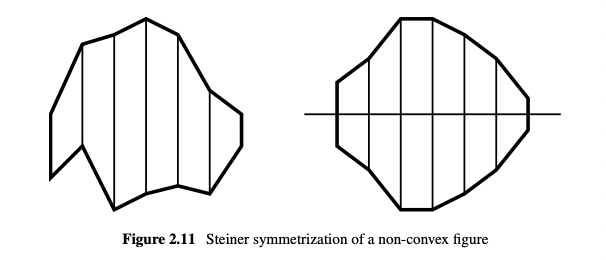
\includegraphics[scale=0.55]{pics/simetrizacion.png}
        %\caption{Caption}
        \label{fig:my_label}
    \end{figure}
    \blfootnote{Imagen obtenida de \cite{book}}
\end{frame}
%AGREGAR FOOTNOTE DE REF
%-----------------------


%-----------------------
\begin{frame}{Simetrización de Steiner}
\textbf{Teorema.}
    \begin{itemize}
        \item $\mathcal{S}(A) \subset \mathcal{S}(B)$ si $A \subset B$.
        \item $\mathcal{S}(A) + \mathcal{S}(B) \subset \mathcal{S}(A+B).$
        \item Si $A$ es convexo, entonces $\mathcal{S}(A)$ es convexo.
        \item La función $\mathcal{S}: \mathcal{K}^n \rightarrow \mathcal{K}^n$ es continua y \textbf{preserva volúmenes}. 
    \end{itemize}
\end{frame}
%-----------------------


%-----------------------
\begin{frame}{Demostración de la DBM}

\textit{Bosquejo (Blaschke):}
\begin{itemize}[<+->]
    \item Sean $r_1, r_2$ y $r_3$ los radios de las bolas con el mismo volumen de $A$, $B$ y $A+B$ respectivamente. Es suficiente demostrar que $r_1 + r_2 \leq r_3.$
    \item Sea $\epsilon > 0$. Entonces existe una sucecion de simetrizaciones tales que 
    $$B(0, r_1-\epsilon) \subset S_{u_m}(\cdots (S_{u_2}(S_{u_1}(A))) \subset B(0, r_1 + \epsilon),$$
    $$B(0, r_2-\epsilon) \subset S_{u_m}(\cdots (S_{u_2}(S_{u_1}(B))) \subset B(0, r_2 + \epsilon),$$
    $$B(0, r_3-\epsilon) \subset S_{u_m}(\cdots (S_{u_2}(S_{u_1}(A+B))) \subset B(0, r_3 + \epsilon),$$
    \item  Luego, $S_{u_m}(\cdots (S_{u_2}(S_{u_1}(A))) + S_{u_m}(\cdots (S_{u_2}(S_{u_1}(B))) \subset S_{u_m}(\cdots (S_{u_2}(S_{u_1}(A+B))).$
    \item Entonces $B(0, r_1 - \epsilon) + B(0, r_2 - \epsilon) \subset B(0, r_3 + \epsilon)$.
    \item Por tanto $r_1 + r_2 \leq r_3 + 3 \epsilon.$
\end{itemize}
    
\end{frame}
%-----------------------

%-----------------------
\begin{frame}{Demostración de la DBM}
La idea principal de la demostración es que se pueden encontrar una serie de direcciones $u_1, \ldots, u_m$ de tal manera que 

$$\vol(A + B) \geq \vol(B(0, r_1) + B(0, r_2)),$$
donde $\vol(A) = \vol(B(0, r_1))$ y $\vol(B) = \vol(B(0, r_2)).$ Esto es equivalente a la DBM. 
    
\end{frame}
%-----------------------

%-----------------------
\begin{frame}{}
    \begin{figure}
        \centering
        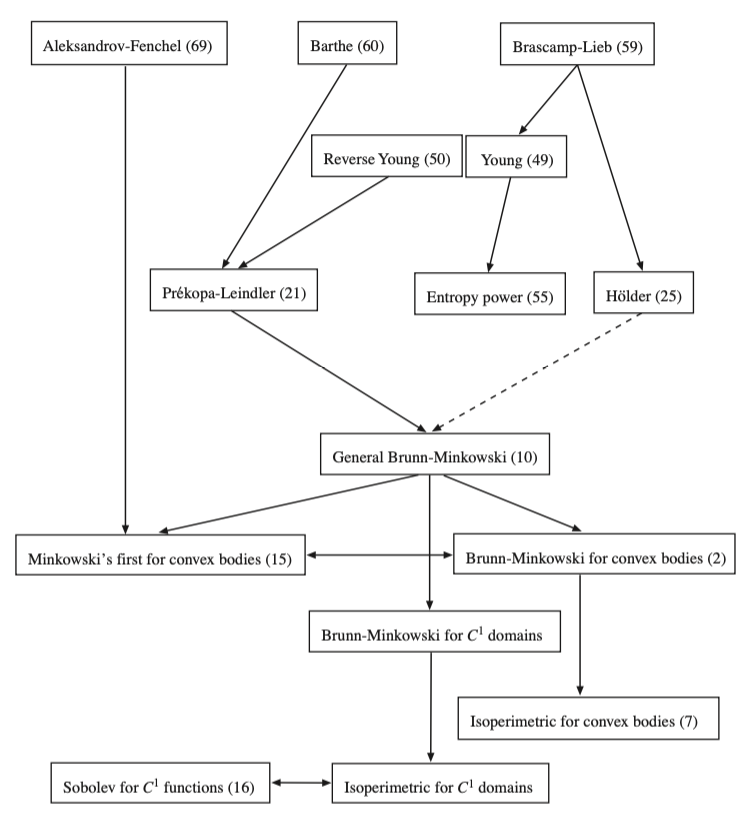
\includegraphics[scale=0.30]{pics/BM-arbol.png}
        %\caption{Caption}
    \end{figure}
    Véase \cite{Gardner2002TheBI} para una exposición completa.
    %\blfootnote{Véase \cite{Gardner2002TheBI} para una }
    %AGREGAR FOOTNOTE DE REF
\end{frame}
%-----------------------


\section{Versiones discretas de la desigualdad de Brunn-Minkowski}
%-----------------------
\begin{frame}{Un primer intento...}
\begin{itemize}[<+->]
    \item Dada la importancia de la DBM en múltiples áreas de las matemáticas, quisiéramos encontrar versiones discretas de esta desigualdad.
    \item Si $A, B$ finitos en $\mathbb{R}^d,$ ¿será cierta la siguiente desigualdad?

    $$\lvert A + B\rvert^{1/d} \geq \lvert A \rvert^{1/d} + \lvert B \rvert^{1/d}. $$
\end{itemize}
    
\end{frame}
%-----------------------


%-----------------------
\begin{frame}{Un primer intento...}

\begin{itemize}[<+->]
    \item Sea $A = \{0\}$ y $B$ cualquier subconjunto finito de $\mathbb R^d$. Note que $A + B = B$. Por tanto  $$ \lvert A + B \rvert^{1/d} = \lvert B \rvert^{1/d} < 1 + \lvert B \rvert^{1/d} = \lvert A \rvert^{1/d} + \lvert B \rvert^{1/d}$$

    \item  Considere $C_{r_1}, C_{r_2}$ cuadrados en $\mathbb R^2.$ Se verifica que:

    $$\lvert C_{r_1} \rvert^{1/2} + \lvert C_{r_2}\rvert^{1/2} = (r_1+1) + (r_2 + 1) > (r_1 + r_2 + 1) = \lvert C_{r_1} + C_{r_2} \rvert^{1/2.} $$

    %DIBUJO
\end{itemize}
\end{frame}
%-----------------------

%-----------------------
\begin{frame}{¿Qué podemos hacer?}
Para obtener resultados discretos análogos a la DBM, podemos:
\begin{itemize}[<+->]
    \item Estudiar subconjuntos $A$ y $B$ con cierta estructura.
    \item Realizar modificaciones a los conjuntos $A,B.$
    \item Buscar resultados análogos a la DBM.

    % CAMBIAR
\end{itemize}
    
\end{frame}
%-----------------------

%-----------------------
%\begin{frame}{Algunas propiedades basicas de cardinalidad... traslacion}
    
%\end{frame}
%-----------------------


%-----------------------
\begin{frame}{Desigualdad trivial}
    En un principio, tenemos la siguiente desigualdad: para $A, B$ subconjuntos finitos de un grupo $G$ libre de torsión, se tiene que 
    $$\lvert A + B\rvert \geq \lvert A \rvert + \lvert B \rvert -1.$$

    La igualdad se satisface cuando $\min \{\lvert A \rvert, \lvert B \rvert\} = 1$ o $A$ y $B$ son \textbf{progresiones aritméticas} con la misma diferencia.

\end{frame}
%-----------------------

%-----------------------
\begin{frame}{Demostración de desigualdad trivial}
\begin{itemize}[<+->]
    \item Como la cardinalidad no cambia por traslaciones, podemos asumir que el máximo de $A$ y el mínimo de $B$ es el origen.
    \item Luego, $A \cap B = \{0\}$ y $A \cup B \subset A + B$, lo que implica que $\lvert A + B \rvert \geq \lvert A \cup B \rvert = \lvert A \rvert + \lvert B \rvert - \lvert A \cap B \rvert = \lvert A \rvert + \lvert B \rvert - 1.$
\end{itemize}
    \begin{figure}
        \centering
        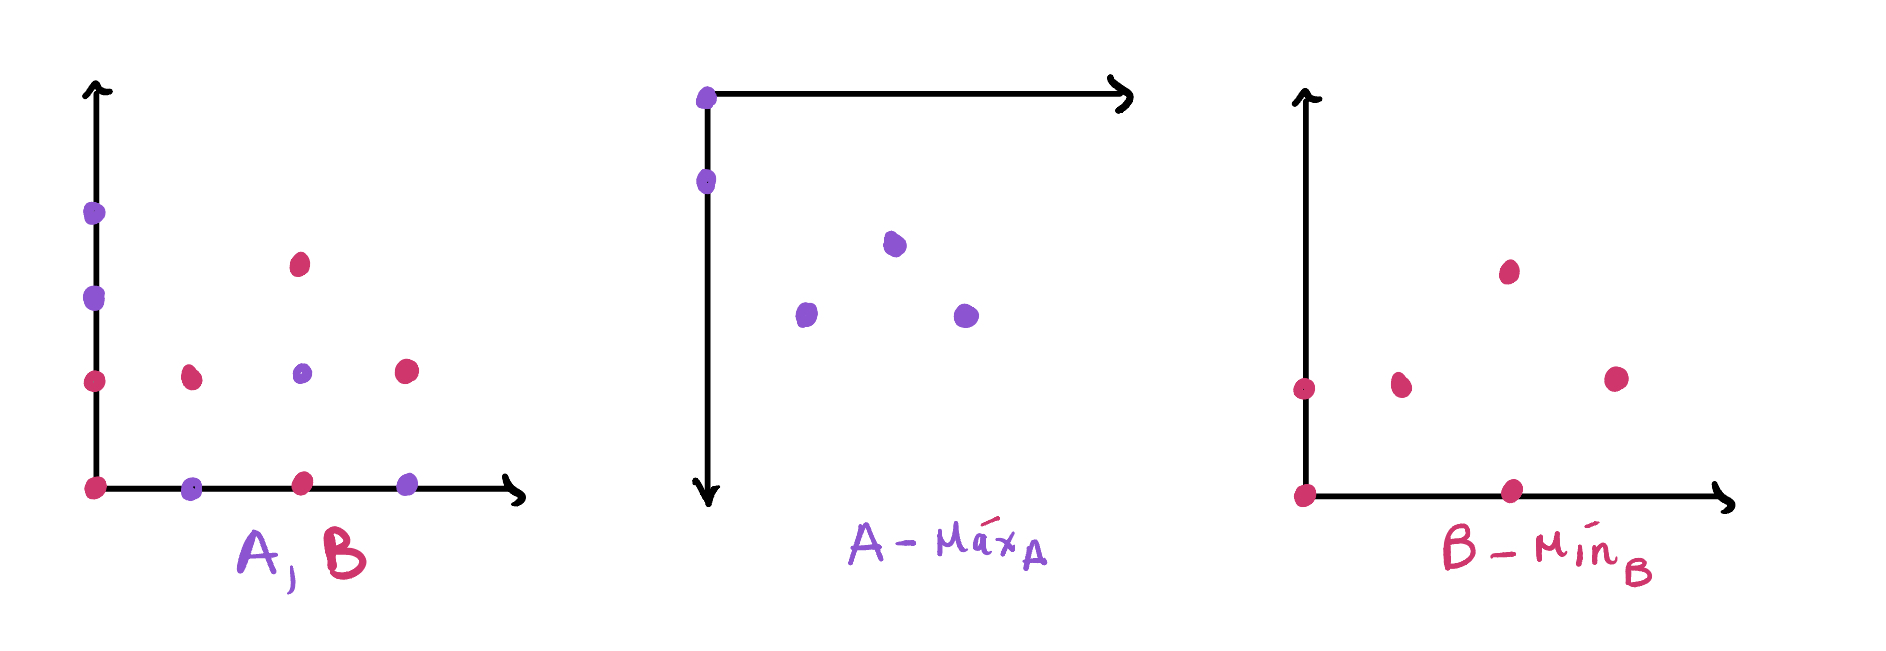
\includegraphics[scale=0.18]{pics/trivial.jpeg}
        %\caption{Caption}
        \label{fig:my_label}
    \end{figure}
\end{frame}
%-----------------------


%-----------------------
\begin{frame}{Resultado de R.J. Gardner y P. Gronchi*}
    \textbf{Teorema} \cite{GardnerGronchi}. Si $A$ y $B$ son subconjuntos finitos de $\mathbb Z^n$ con $dim B = d$, entonces
    $$\lvert A + B \rvert \geq \lvert D^{B}_{\lvert A \rvert} + D^{B}_{\lvert B \rvert} \rvert,$$
    donde $D^B_{\lvert A \rvert}$ y $D^B_{\lvert B \rvert}$ tienen la misma cardinalidad de $A$ y $B$ resp.\\
    \text{ }
    
    \visible<2->{
    Similar al resultado 
    $$\vol(A + B) \geq \vol(B(0, r_1) + B(0, r_2)).$$
}
    
\end{frame}
%-----------------------


%-----------------------
\begin{frame}{Resultado de R.J. Gardner y P. Gronchi*}
Como corolarios al resultado anterior, se obtienen las siguientes desigualdades del tipo DBM:
\begin{itemize}
    \item Si $A, B$ son subconjuntos finitos de $\mathbb R^d$, con $\lvert B \rvert \leq \lvert A \rvert$ y $dim B = n$, entonces $$\lvert A + B \rvert \geq \lvert A \rvert + (d-1) \lvert B \rvert + (\lvert A \rvert - d)^{(d-1)/d}(\lvert B \rvert - d)^{1/d} - \frac{d(d-1)}{2};$$
    \item Si $A, B$ son subconjuntos finitos de $\mathbb R^d$ con $dim B = n$,$$\lvert A + B \rvert^{1/d} \geq \lvert A \rvert^{1/d} + \frac{1}{(d!)^{1/d}} (\lvert B \rvert - d)^{1/d}$$
\end{itemize}
\end{frame}
%-----------------------


%-----------------------
\begin{frame}{Resultado de T. Tao y B. Green*}
    \textbf{Teorema }\cite{https://doi.org/10.48550/arxiv.math/0511069}. Suponga que $A$ y $B$ son subconjuntos finitos de $\mathbb R^k$. Entonces, para toda $d \leq k$ tenemos que
    $$\lvert A + B + \{0,1\}^d \rvert \geq  2^{d} \min \left(\lvert A \rvert, \lvert B \rvert \right),$$
    donde encajamos a $\mathbb Z^d$ en $\mathbb R^k$ de manera obvia.\\
    \text{}

    \visible<2->{
    Similar al resultado 
    $$\vol(A + B) \geq 2^d \min\{\vol(A),\vol(B)\}.$$
}
\end{frame}
%-----------------------


%-----------------------
%\begin{frame}{Otros resultados}
%\begin{itemize}
 %   \item Para $A,B \subset \mathbb Z^d$ finitos, se tiene $\lvert \overline{A} + B \rvert^{1/d} \geq \lvert A \rvert^{1/d} + \lvert B \rvert^{1/d}.$
  %  \item Para $A,B \subset \mathbb Z^d$ finitos, se tiene $\lvert A + B \rvert^{1/d} \geq \lvert r(A) \rvert^{1/d} + \lvert B \rvert^{1/d}.$
%\end{itemize}    
%\end{frame}
%-----------------------


\section{Proyecciones y cardinalidad del conjunto suma}

%-----------------------
\begin{frame}{Proyecciones y cubiertas}
\begin{itemize}[<+->]
    \item Sea un subespacio de $\mathbb R^d.$ Denotaremos por $\phi_H: \mathbb R^d \rightarrow \mathbb R^d/H$ la proyección natural modulo $H$.
    \item Denotaremos por $h_{d-1}(A,B)$ al mínimo entero $s$ tal que existen hiperplanos $H_1,\ldots, H_s, H^\prime_1, \ldots, H^\prime_s$ con $A \subset \bigcup_{i=1}^s H_i$ y $B \subset \bigcup_{i=1}^s H^\prime_i.$
    \item Alternativamente, se puede ver que $h_{d-1}(A, B)$ es la mínima $s$ tal que existe un hiperplano $H$ de que cumple que $\lvert \phi_H(A)\rvert, \lvert \phi_H(B) \rvert \leq s.$
\end{itemize}
    
\end{frame}
%-----------------------


%-----------------------
\begin{frame}{Proyecciones y cubiertas}
    \begin{figure}
        \centering
        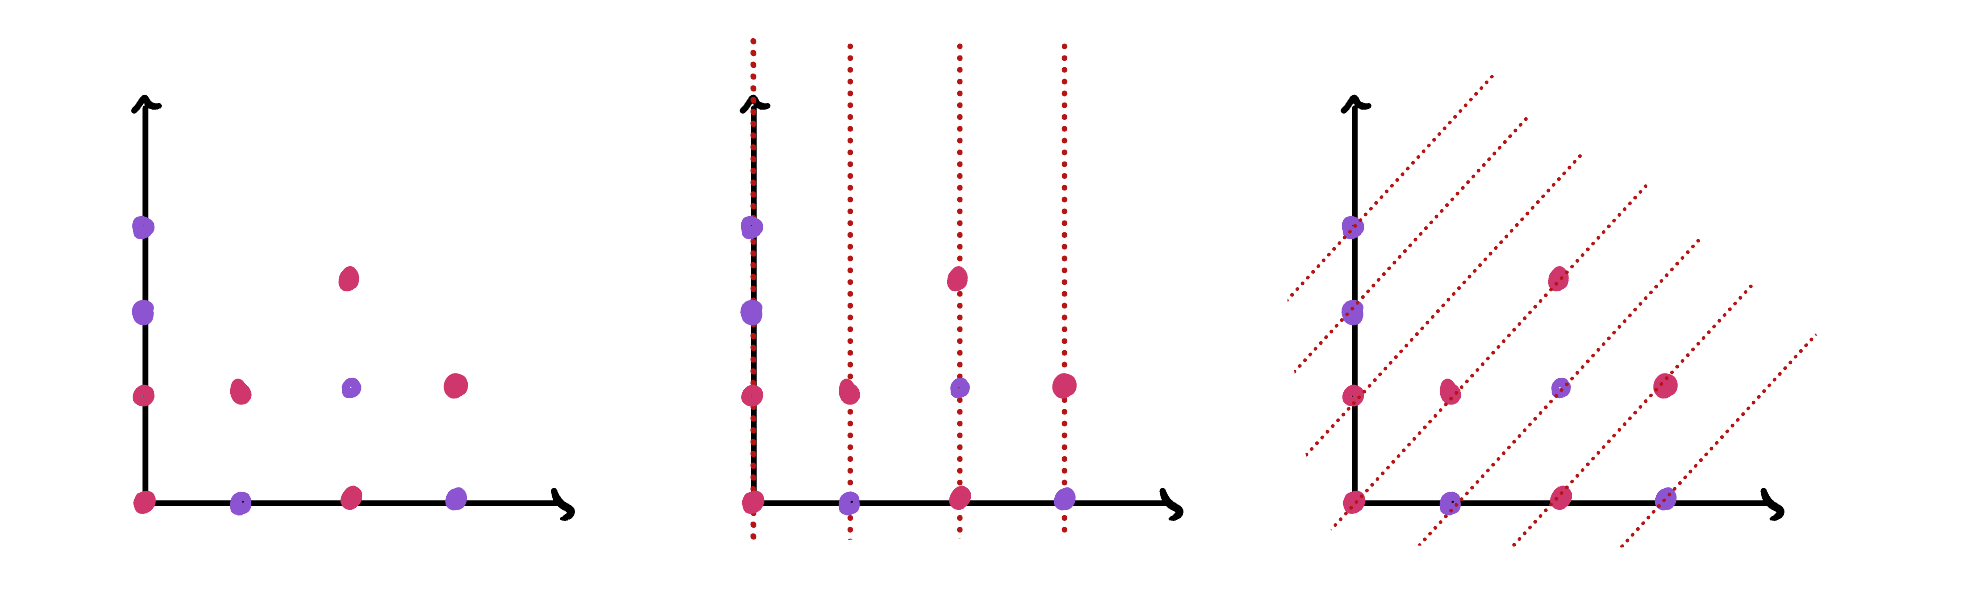
\includegraphics[scale=0.17]{pics/proyeccion.jpeg}
        \caption{Los conjuntos $A$ y $B$ representados con colores distintos. En este ejemplo se tiene que $h_1(A,B) = 4$}
        %\label{fig:my_label}
    \end{figure}
\end{frame}
%-----------------------




%-----------------------
\begin{frame}{Teorema $2^d$ de Freiman}
\textbf{Teorema} \cite{Freimanbook}.
    Sea $d \geq 2$ un entero y sea $0 < c < 2^d.$ Existen constantes $k = k(c,d)$ y $s = s(c,d)$ tales que si $A \subset \mathbb R^d$ es finito, distinto del vacío y satisface que $\lvert A \rvert \geq k$ y $\lvert A + A \rvert < c \lvert A \rvert $, entonces $h_{d-1}(A, A) < s.$
\visible<2->{
$$\lvert A + A \lvert < c \lvert A \rvert \ \text{(la suma es pequeña)} \Rightarrow $$
$$ A \text{ es cubierto por menos de } s \text{ hiperplanos } (A \text{ tiene estructura}) $$
}

\end{frame}
%-----------------------

%-----------------------
\begin{frame}{Teorema $2^d$ de Freiman}
    El Teorema $2^d$ de Freiman nos sugiere que la cardinalidad de $A$ y $B$, modulo ciertos subespacios, tienen un papel importante en la cardinalidad de la suma $A + B.$
\end{frame}
%-----------------------


%-----------------------
\begin{frame}{Resultado de D. Grynkiewicz y O. Serra}
    \textbf{Teorema} \cite{GRYNKIEWICZ2010164}. Sean $A, B \subset \mathbb R^2$ finitos y distintos del vacío. Sea $l = \mathbb R x_1$ una línea, $m$ el número de líneas paralelas a $l$ que intersectan a $A$ y $n$ el número de líneas paralelas a $l$ que intersectan a $B$. Entonces

    $$\lvert A + B \rvert \geq \left( \frac{\lvert A \rvert}{m} + \frac{\lvert B \rvert}{n} \right) (m+n-1). $$

    %% DIBUJO
\end{frame}
%-----------------------

\begin{frame}{}
    \begin{figure}
        \centering
        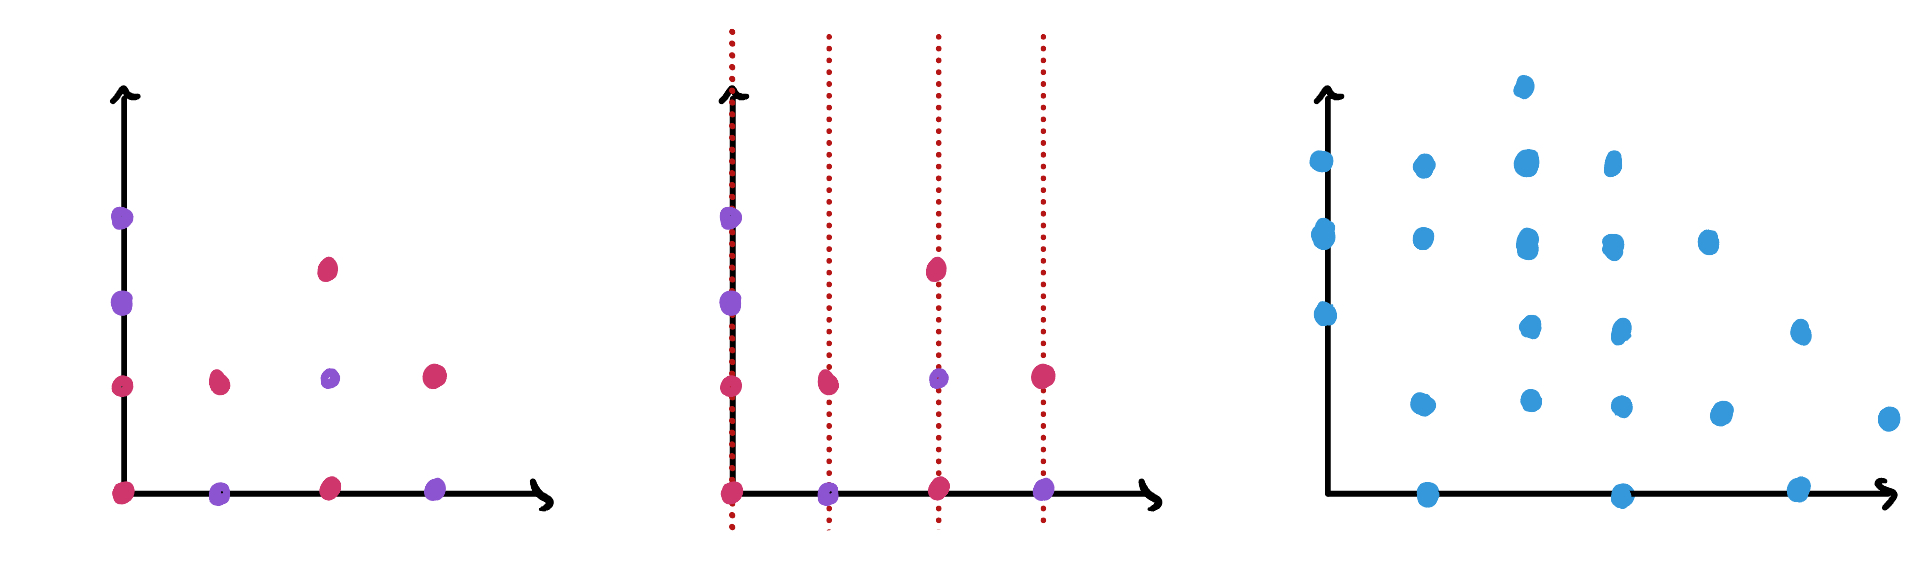
\includegraphics[scale=0.15]{pics/gryn.jpeg}
        %\caption{Caption}
        %\label{fig:my_label}
    \end{figure}

    En este ejemplo, $\lvert A \rvert = 5$, $\lvert B \rvert = 6$, $\lvert A + B \rvert = 22$  y $n = 4 = m$. Note que 
    \begin{equation*}
        (m+n-1) \left( \frac{\lvert A \rvert}{m} + \frac{\lvert B \rvert}{n} \right) = 7\cdot \left(\frac{11}{4}\right) < \lvert A + B \rvert. 
    \end{equation*}
\end{frame}


%-----------------------
\begin{frame}{Compresión lineal}
    Sea $X = (x_1, \ldots, x_d)$ una base ordenada de $\mathbb R^d$. Para un conjunto finito $A \subset \mathbb R^d$, definimos la \textbf{compresión lineal} de $A$ respecto a $x_i \in X$, como el conjunto $C_i(A)$, definido a trozos como sigue:

    $$\phi_{H}(C_i(A) \cap (\mathbb R x_i + a )) = \{0, x_i, 2x_i, \ldots, (r-1) x_i\},$$
    donde $H = \langle x_1, \ldots x_{i-1}, x_{i+1}, \ldots, x_d \rangle$, $r = \lvert A \cap (\mathbb R x_i + a) \rvert$ y el lado derecho de la ecuación es vacío si $r=0.$ Definimos la \textbf{compresión total} de $A$

    $$C_X(A) = C_d((C_{d-1}(\ldots (C_1(A)).$$

    \blfootnote{Todos los resultados anteriores utilizaron compresión.}
\end{frame}
%-----------------------


%-----------------------
\begin{frame}{Compresión lineal}
    \begin{figure}
        \centering
        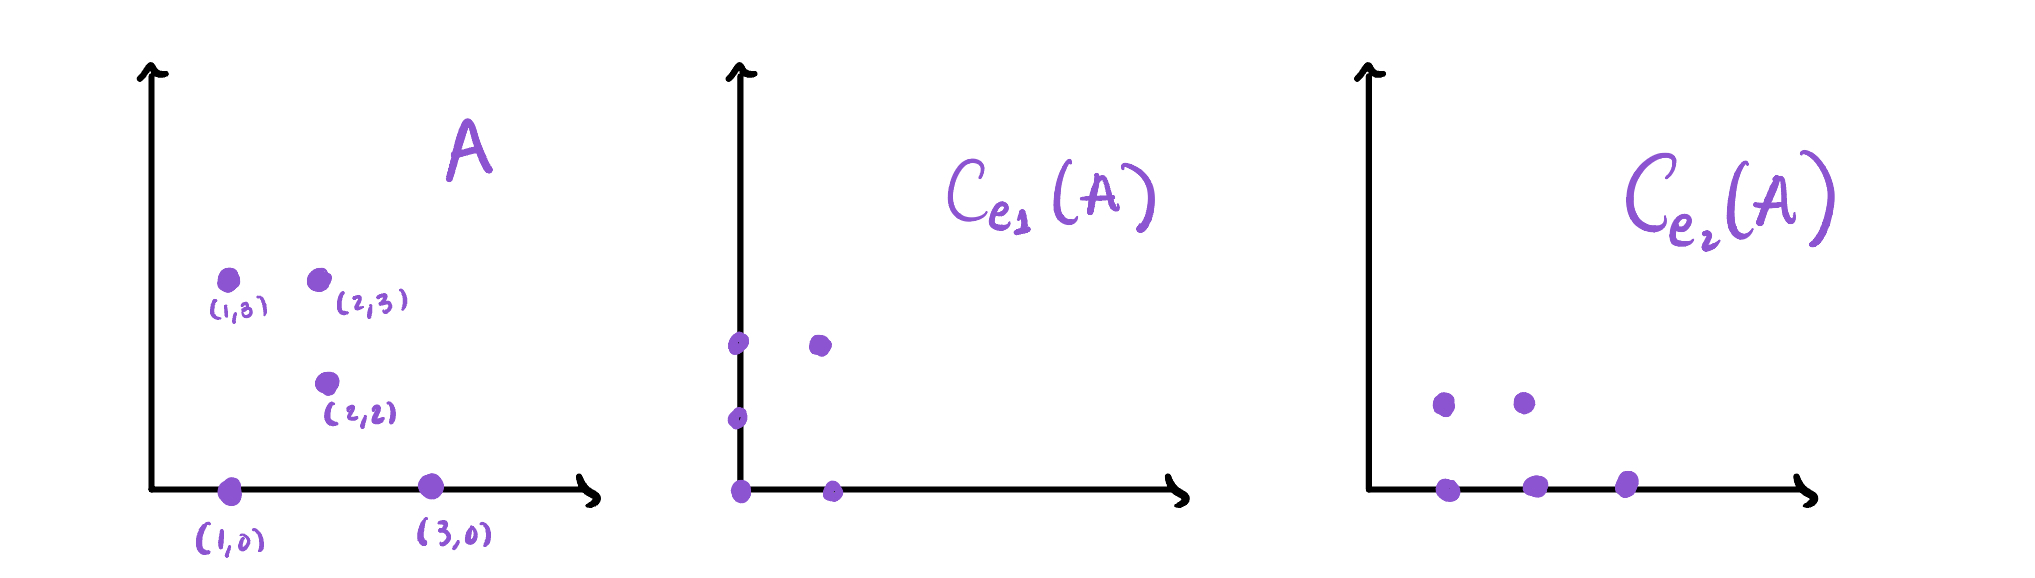
\includegraphics[scale=0.16]{pics/compresion.jpeg}
        \caption{Compresión del conjunto $A$ (izq.), en la dirección $e_1$ (centro) y en la dirección $e_2$ (dcha).}
    \end{figure}
\end{frame}
%-----------------------


%-----------------------
\begin{frame}{Compresión lineal}
    \begin{figure}
        \centering
        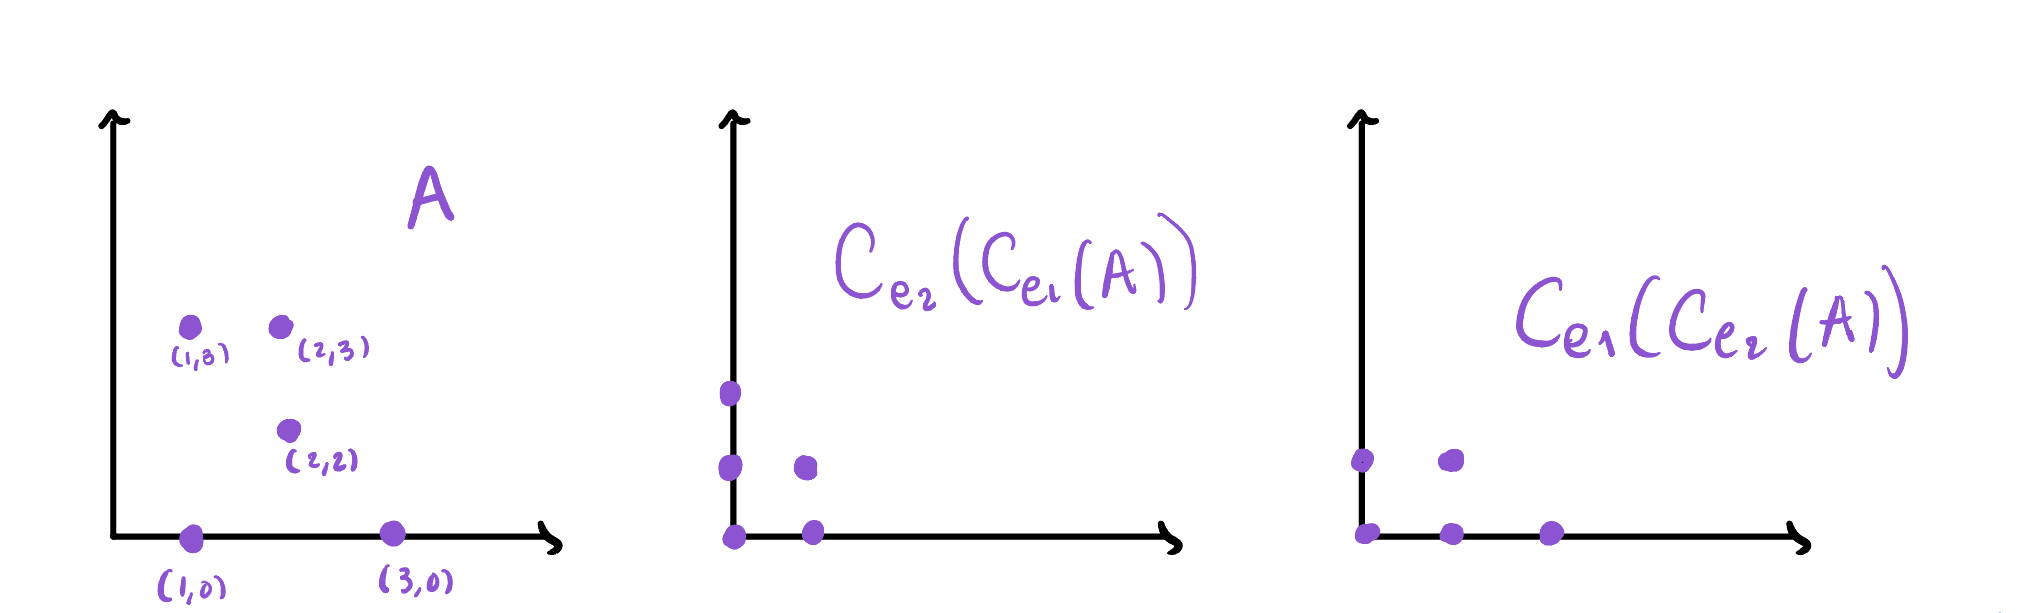
\includegraphics[scale=0.16]{pics/compresion2.jpeg}
        \caption{Compresión total de $A$ (izq.) respecto a la base $\{e_1, e_2\}$ en distintos órdenes.}
      
    \end{figure}
\end{frame}
%-----------------------

\begin{frame}{Compresión lineal}
\textbf{Observación:} 
    \begin{eqnarray*}
    \lvert A + B \rvert &=& \sum_{t \in H} \lvert (A + B)_t \rvert\\
    &\geq& \sum_{t\in H} \max\{\lvert A_s + B_{t-s}\rvert: A_s \neq \varnothing, B_{t-s} \neq \varnothing\}\\
    &\geq& \sum_{t\in H} \max \{\lvert A_s \rvert + \lvert B_{t-s}\rvert: A_s \neq \varnothing, B_{t-s} \neq \varnothing \} \\
    &=& \lvert C_i(A) + C_i(B) \rvert.
    \end{eqnarray*}
    Por lo que 
    $$\lvert A + B \rvert \geq \lvert C_X(A) + C_X(B) \rvert.$$
\end{frame}
%-----------------------


%-----------------------
\begin{frame}{Demostración del resultado de D.Grynkiewicz y O. Serra}
    \begin{itemize}
        \item Por la observación anterior, se tiene que $\lvert A + B \rvert \geq \lvert C_X(A) + C_X(B) \rvert.$
        \item $\lvert C_X(A) + C_X(B) \rvert = \sum_{l=2}^{m+n} \max_{i}\{a_i + b_{l-i}: 1 \leq i \leq m, 1 \leq l-i \leq n\} - (m+n-1)$.
        \item $\frac{1}{m+n-1} \sum_{l=2}^{m+n} \max_{i}\{a_i + b_{l-i}: 1 \leq i \leq m, 1 \leq l-i \leq n\} \geq \frac{1}{m}\sum_{i=1}^m a_i + \frac{1}{n} \sum_{i=1}^n b_i.$
    \end{itemize}
\end{frame}
%-----------------------

%-----------------------
\begin{frame}{¿Cuándo se satisface la igualdad?}
    Siempre que tengamos \textbf{trapezoides} \cite{Freiman_2012}.
    \begin{figure}
        \centering
        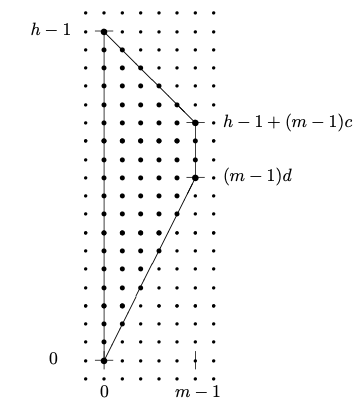
\includegraphics[scale=0.5]{pics/trapecios.png}
     
    \end{figure}
\end{frame}
%-----------------------


%-----------------------
\begin{frame}{Desigualdad de Bonneson}
    \textbf{Teorema} .Si $A, B \subset \mathbb R^d$ son compactos y $H \subset \mathbb R^d$ es un hiperplano, entonces
    $$\vol(A+B) \geq \left(M^{1/(d-1)} + N^{1/(d-1)} \right)^{d-1} \left(\frac{\vol(A)}{M} + \frac{\vol(B)}{N} \right), $$
    donde $M = \sup\{\vol((x + H) \cap A): x \in \mathbb R^d\}$ y $N = \sup\{\vol((x + H) \cap B): x \in \mathbb R^d\}.$ \\

    \text{ }
    \visible<2->{
    Se puede demostrar que la anterior desigualdad también es válida cuando $M = \vol(\varphi(A))$, $N = \vol(\varphi(B))$, donde $\varphi: \mathbb R^d \rightarrow H$ es la proyección en el hiperplano $H.$
    }
\end{frame}
%-----------------------

%-----------------------
\begin{frame}{¿Qué pasa en otras dimensiones?}
        \small¿Será cierta la siguiente desigualdad?
        $$\lvert A + B \rvert \geq \left(\frac{\lvert A \rvert}{a_1}  + \frac{\lvert B \rvert}{b_1} - 1\right) \left(\frac{a_1}{a_2} + \frac{b_1}{b_2} - 1 \right) \left(a_2 + b_2 -1 \right),$$
        donde $a_1$ y $b_1$ es el número de líneas paralelas al eje $x$ que intersectan a $A$ y $B$ respectivamente; y $a_2$ y $b_2$ es el número de planos paralelos al plano $xy$ que intersectan a $A$ y $B$ respectivamente.

\end{frame}
%-----------------------



%-----------------------
\begin{frame}{Conjetura de Grynkiewicz}
    \textbf{Conjectura} \cite{alma9941126213902959}. Sean $A, B \subset \mathbb{R}^d$ finitos y distintos del vacío. Sea $X = \{x_1,\ldots, x_d\}$ una base para $\mathbb R^d$. Entonces existe una permutación $\sigma$ de $\{1,\ldots, d\}$ tal que 
    $$\lvert A + B \rvert \geq \prod_{i=1}^d \left( \frac{\lvert \phi_{X_{i-1}}(A) \rvert}{\lvert \phi_{X_i}(A) \rvert} + \frac{\lvert \phi_{X_{i-1}}(B) \rvert}{\lvert \phi_{X_i}(B) \rvert} - 1 \right),$$
    donde $X_i = 0 + \mathbb R x_{\sigma(1)} + \cdots \mathbb R x_{\sigma(i)}$ para $i = 0, \ldots, d.$
\end{frame}
%-----------------------


%-----------------------
%\begin{frame}{?Algunos resultados propios}
    
%\end{frame}
%-----------------------



%-----------------------
\begin{frame}{Referencias}
\small
\printbibliography
\end{frame}
%-----------------------

%-----------------------
\begin{frame}{}
\centering
    \Large ¡MUCHAS GRACIAS!
\end{frame}
%-----------------------

\end{document}